\documentclass[a4paper, 11p]{article}
\usepackage{tgtermes}

\usepackage{biblatex}
\addbibresource{reffs.bib}

\usepackage{listings}
\usepackage{enumitem}
\usepackage{amsmath, amssymb, mathtools}

\usepackage{graphicx}

\usepackage{geometry}
\geometry{margin=.6in}

\begin{document}

\begin{titlepage}
    \centering
    \LARGE

    \vspace*{.5in}
    \textbf{Ministry of Education and Research of the Republic of Moldova} \\
    \textbf{Technical University of Moldova} \\
    
    \vspace*{.2in}
    \textbf{Department of Software Engineering and Automation} \\
    
    \vspace*{1in}
    { \Huge
      \textbf{REPORT}}

    \vspace*{.3in}
    \textbf{Laboratory work No 1} \\
    \textbf{at Computer Programming} \\
    
    \vfill
    { \raggedright
        \textbf{Performed by:} \\
        st. gr. FAF-233 \hfill A. Chicu \\
        
        \vspace*{1cm}
        \textbf{Verified by:} \\
        dr., conf. univ. \hfill M. Kulev \\
    }
    
    \vfill

    Chișinău -- 2023 
    
\end{titlepage}

\begin{center}
   \Large
   \textbf{Laboratory work no 1} \\
   \textbf{Topic:} Using control instructions and cyclic statements in the C language
\end{center}

\section{Purpose of the laboratory work:}
Study techniques and methods of using 
condition control instructions and cyclic instructions in 
C language for function tabulation. 

\section{Problem condition:}
Calculate and display at 
screen the values of the argument x and the values of the function F, defined by 3 
given expressions, for the interval \( x_1 \le  x \le  x_2 \) and the step \( p_x \) of 
increment of the argument \( x \). The values \( x_1, x_2, p_x \) and the parameters \( a, b, c \) are real input data.

\section{Calculation formulas \textit{(variant 6)}}
\begin{align*}
F = 
\begin{dcases}
    \frac{1 + x}{x - \cos c} - \frac{b}{a} & \text{if } b - a < 0 \text{ and } c = o \\
    \frac{a - bx}{\ln x} & \text{if } b - a > 0 \text{ and } c \neq 0 \\
    \frac{10x + 2}{c^2x - 6 -b} & \text{in all other cases}
\end{dcases}
\end{align*}

\vspace*{.2in}
\begin{center}
    \Large \textbf{Laboratory work processing:}
\end{center}

\setcounter{section}{4}

\subsection{ Short theory on laboratory work topic:} 
In Computer Programming \cite{progsgh} control instructions are commands that manage the flow of a program, determining which parts execute under specific conditions.

Cyclic statements, like loops, are a subset of control instructions used to repeat code execution until certain conditions are met, facilitating efficient repetition. Together, they enable precise control and automation within computer programs.
\begin{enumerate}
    \item \textbf{While Loop:} The while loop in programming is a cyclic statement that repeatedly executes a block of code as long as a specified condition remains true. It checks the condition before entering the loop.
    \item \textbf{Do-While Loop:} The do-while loop is similar to the while loop but with the difference that it executes the code block first and then checks the condition. This means that the code block will run at least once, even if the condition is initially false.
    \item \textbf{Goto Statement:} The goto statement is a control transfer statement that allows you to jump to a labeled section of code. It's generally discouraged in modern programming because it can lead to unreadable and error-prone code. It's often considered a less structured way to control program flow.
    \item \textbf{Conditional Statements:} \textbf{if} and \textbf{else} are control instructions used for decision-making in a program. 
        \textbf{if} allows you to execute a block of code if a specified condition is true.
        \textbf{else} provides an alternative block of code to execute if the condition in the \textbf{if} statement is false.
        Together, they allow a program to take different actions based on different conditions.
\end{enumerate}
\pagebreak

\subsection{Description of data (variables): }
\begin{enumerate}[label=\alph*)]
    \item \textbf{Input data:}  
        \begin{itemize}
            \item \texttt{x1}, \texttt{x2}, and \texttt{px}: These are input values entered by the user to specify the range of x values and the step size between them. \textit{(of real type)}
            \item \texttt{a}, \texttt{b}, and \texttt{c}: These are input values entered by the user for the mathematical calculations. \textit{(of real type)}
        \end{itemize}
        The variables above are then carried to each of the functions representing a cycle type.

    \item \textbf{Output data:} \\
        The output of this code is a series of calculations for different values of x within the specified range. The output includes:
        \begin{itemize}
            \item \texttt{n}: The iteration number. \textit{(of integer type)}
            \item \texttt{x}: The current value of \texttt{x}. \textit{(of real type)}
            \item \texttt{res}: The result of the function \texttt{F()} for the given inputs. \textit{(of real type)}
        \end{itemize}
        These values are printed to the console for each cycle type at every iteration.

    \item \textbf{Working data:}
        \begin{itemize}
            \item \texttt{res}: This variable is used to store the result of the function \texttt{F()} within each loop iteration. \textit{(of real type)}
            \item \texttt{n}: This variable is used to keep track of the iteration number. \textit{(of integer type)}
            \item \texttt{x}: This variable is used to store the current value of \texttt{x} within the loop. \textit{(of real type)}
        \end{itemize}
\end{enumerate}
\pagebreak

\subsection{Algoritm desctiption\cite{diagrams}}
\begin{figure}[!h]
  \centering
  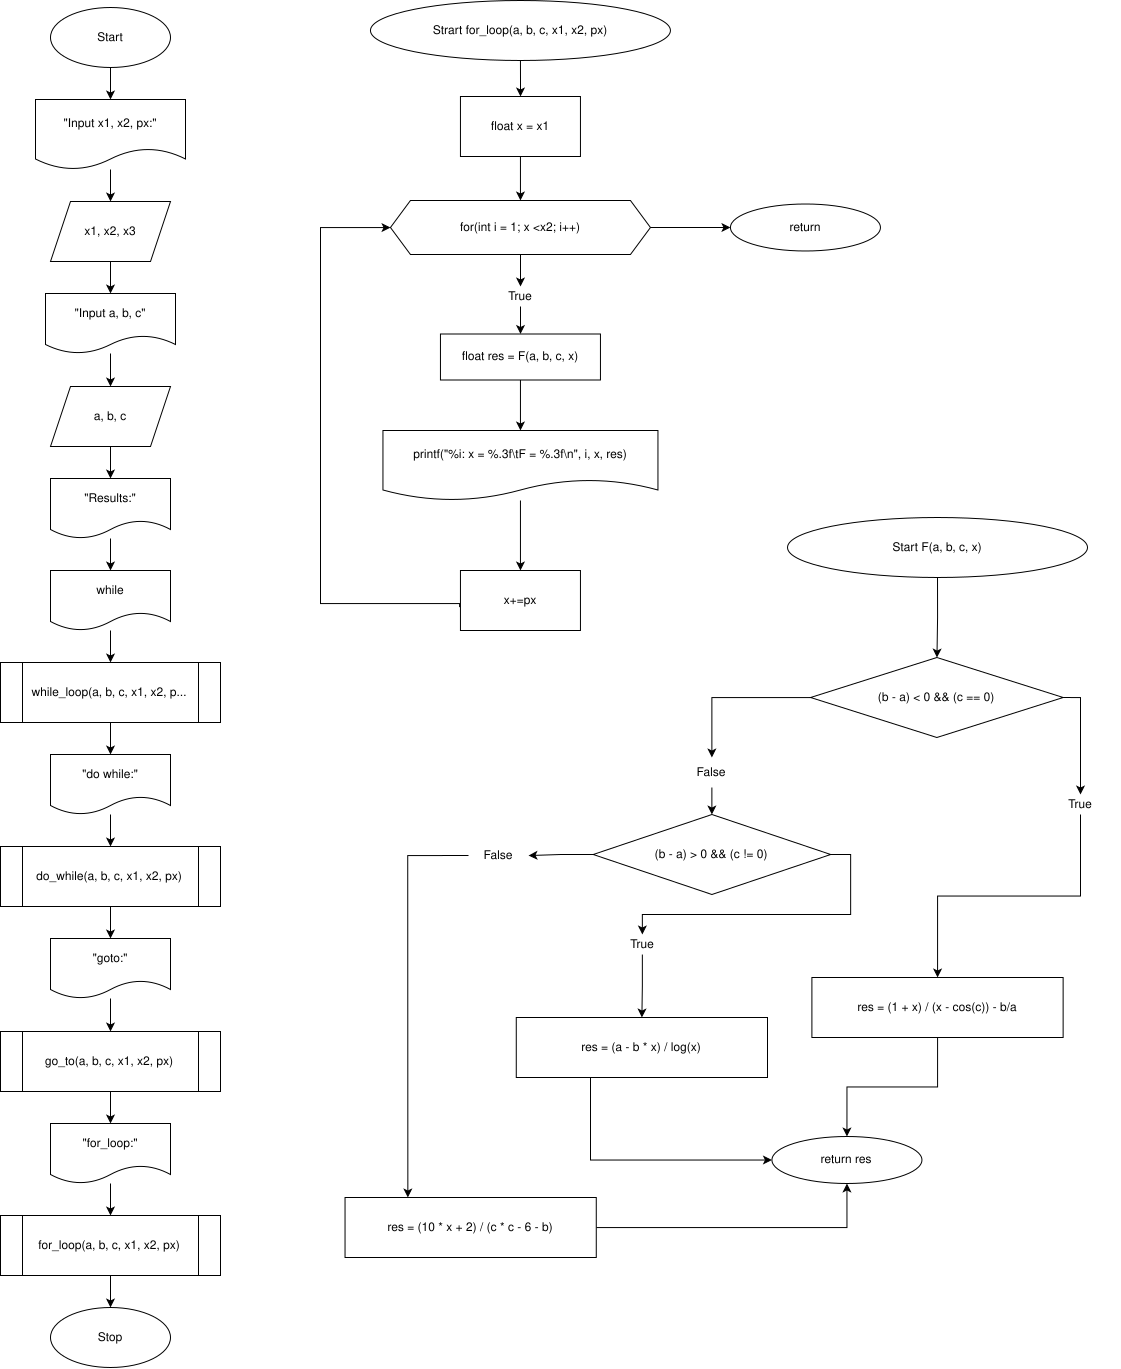
\includegraphics[width=\textwidth]{flowchart.png}
  \caption{Flowchart}
\end{figure}
\pagebreak

\subsection{Program code (text) in C language (listing of the program): }
\lstset{
  basicstyle=\ttfamily,
  language=C,                % choose the language of the code
  numbers=left,                   % where to put the line-numbers
  stepnumber=1,                   % the step between two line-numbers.        
  numbersep=5pt,                  % how far the line-numbers are from the code
  showspaces=false,               % show spaces adding particular underscores
  showstringspaces=false,         % underline spaces within strings
  showtabs=false,                 % show tabs within strings adding particular underscores
  tabsize=2,                      % sets default tabsize to 2 spaces
  breaklines=true,                % sets automatic line breaking
  breakatwhitespace=true,         % sets if automatic breaks should only happen at whitespace
  title=\lstname,                 % show the filename of files included with \lstinputlisting;
}
\lstinputlisting{main.c}

\subsection{Results of running and testing the program (screenshot):}
\begin{figure}[!h]
  \centering
  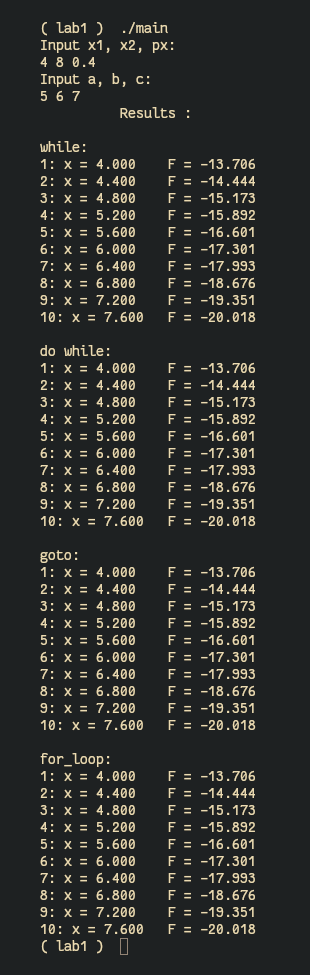
\includegraphics[width=2in]{output.png}
  \caption{output}
\end{figure}
\pagebreak

\subsection{Verification of the results\cite{testlabs}:}
\begin{figure}[!h]
  \centering
  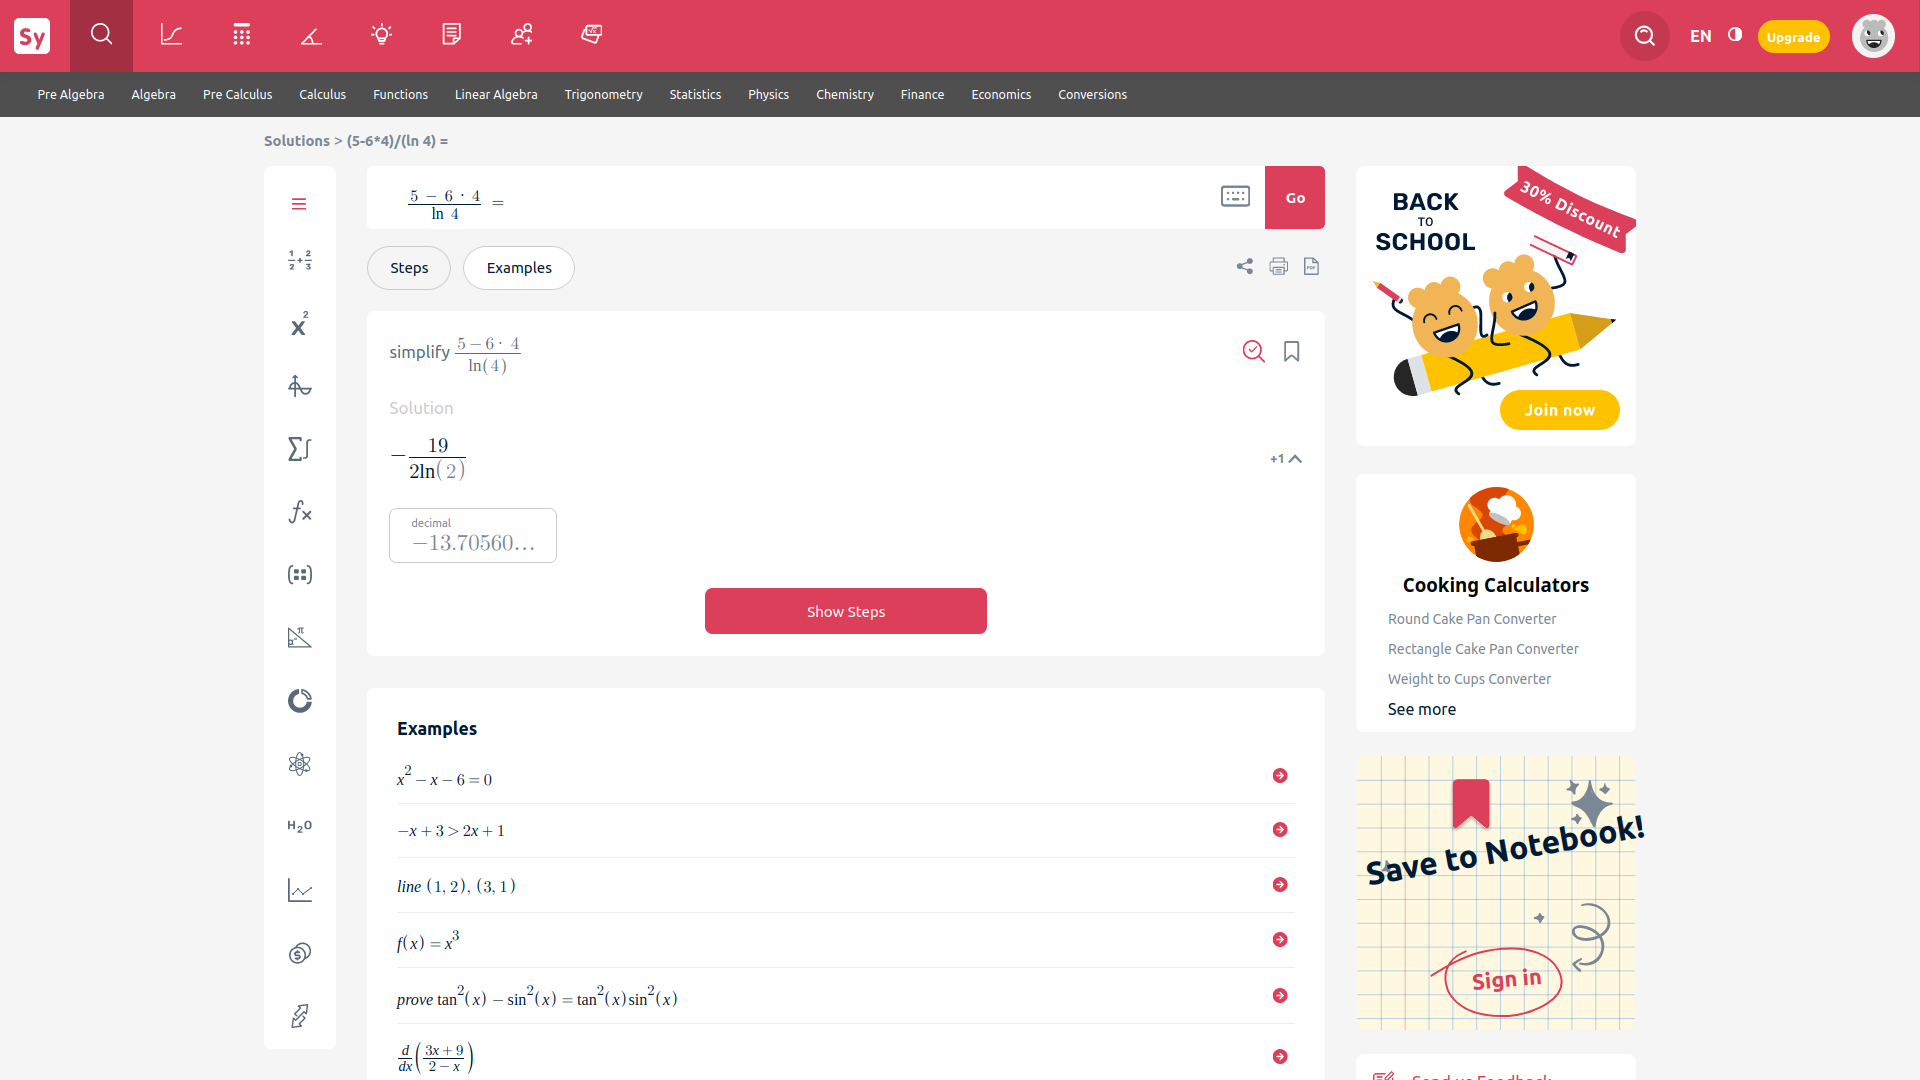
\includegraphics[width=6in]{verif_1.png}
  \caption{for \( x = 4.00 \)}
\end{figure}

\begin{figure}[!h]
  \centering
  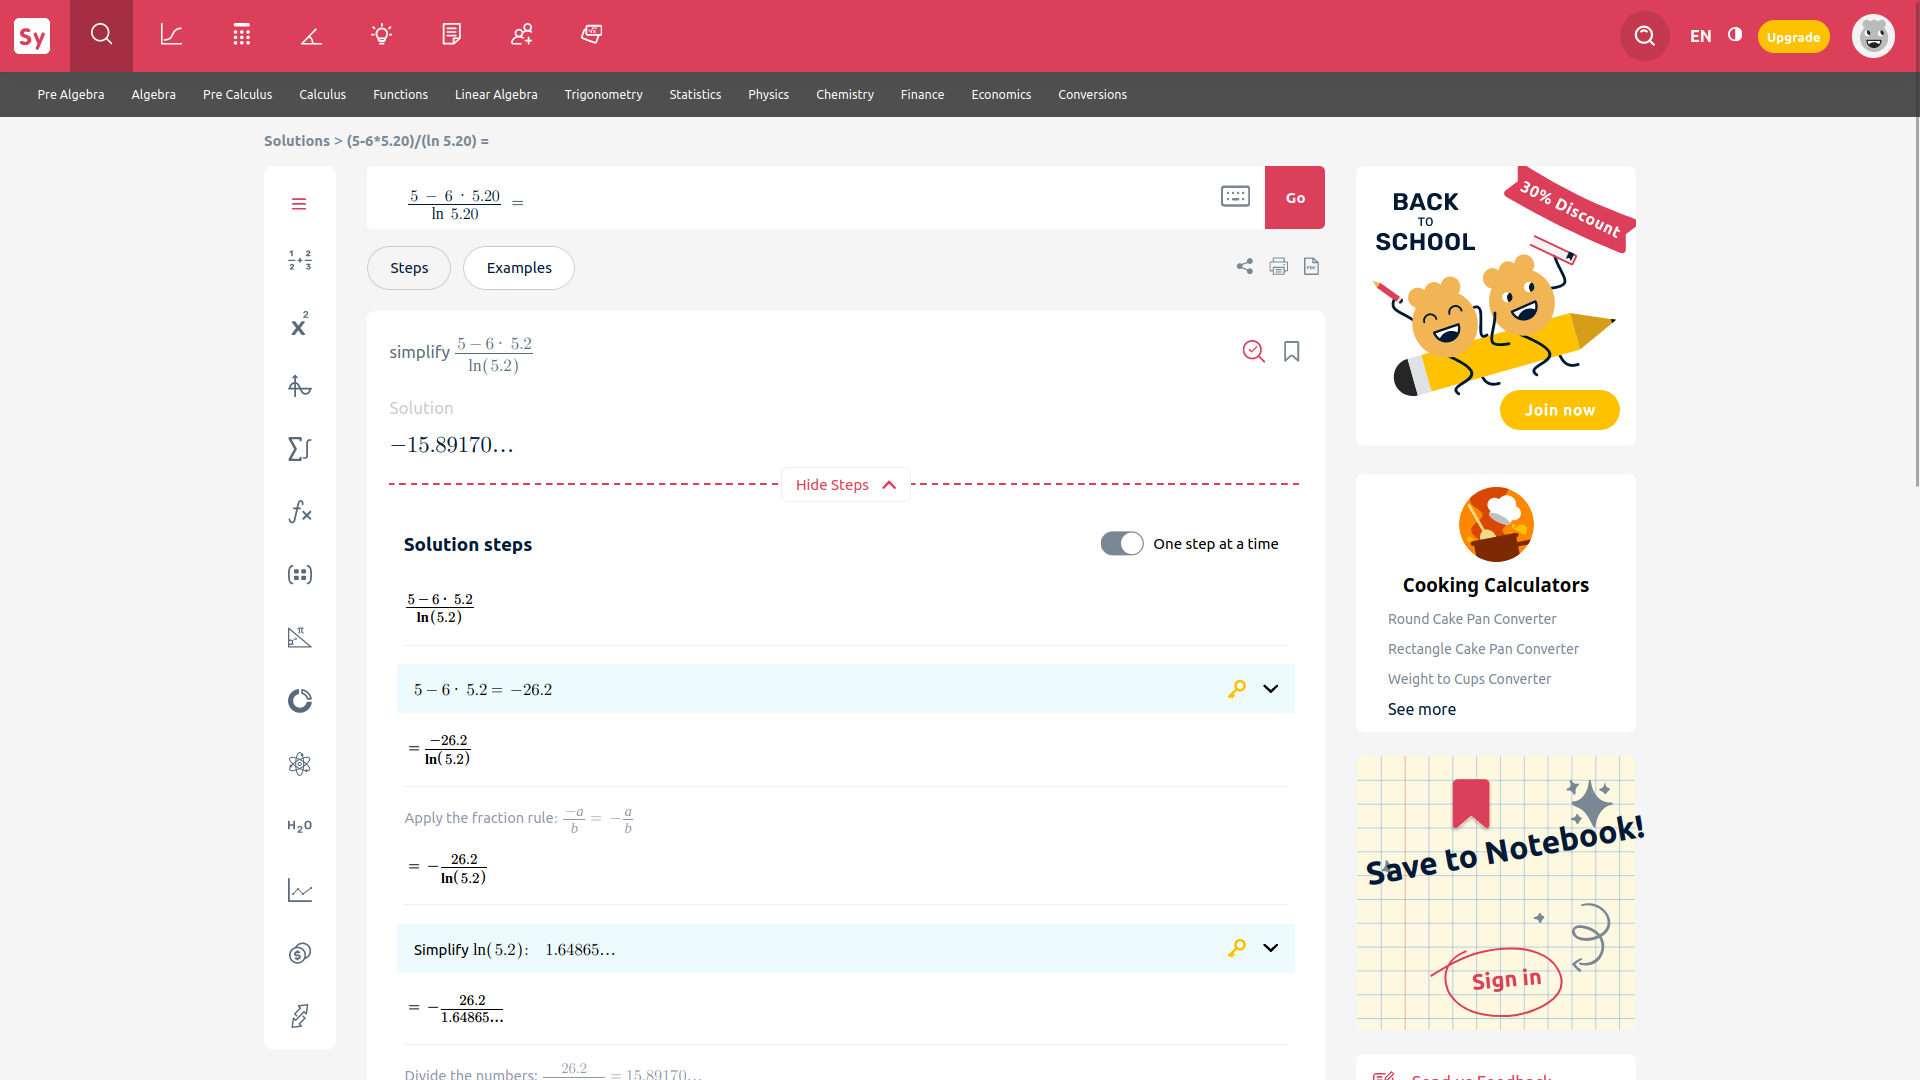
\includegraphics[width=6in]{verif_2.png}
  \caption{for \( x = 5.20 \)}
\end{figure}

\begin{figure}[!h]
  \centering
  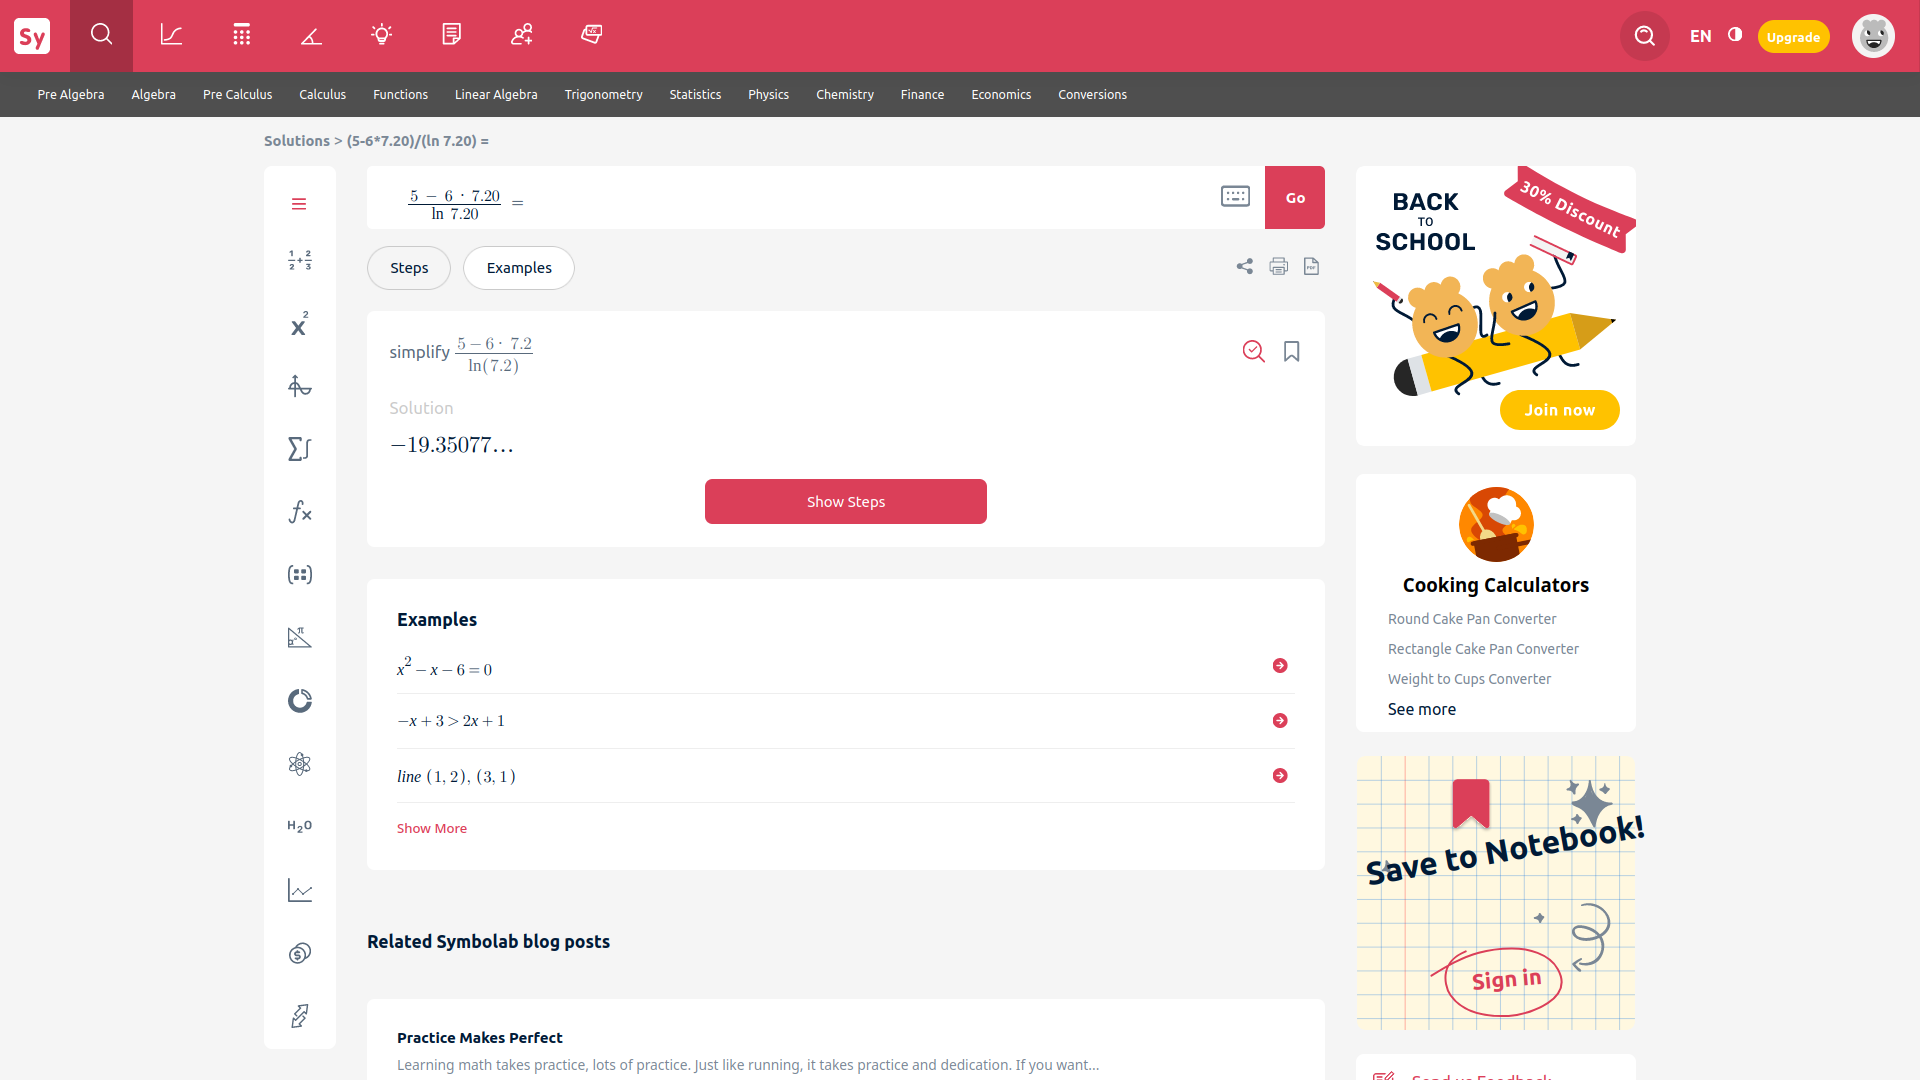
\includegraphics[width=6in]{verif_3.png}
  \caption{for \( x = 7.20 \)}
\end{figure}

\pagebreak

\subsection{Analysis of results and conclusions: }
\begin{enumerate}
 
    \item Have been developed skills to compile, run and test a simple program in the C programming language. 
    \item The verification of the results confirms that the elaborated program works correctly. 
    \item Control instructions can be used to represent complex formulas.
    \item Cyclic statements allow for iterating over a range of values to obtain function results which may be used in the future in plotting a graph.
    \item When implementing the \texttt{go\_to()} subprogram, I have received some errors initially.
    \item The developed program can be further improved by defining and referencing to global variables instead of passing down \texttt{x1, x2, px, a, b, c} to every subprogram.
    
\end{enumerate}

\printbibliography

\end{document}
